\section{Related Work}

\subsection{Transformers in Offline \acrshort{rl}}

\subsubsection{Trajectory Transformer}
\sloppy The Trajectory Transformer trains on sequences of transitions $(state, action, reward)$ and it repurposes beam search as a reward-maximizing strategy \cite{trajectory_transformer}. The Decision Transformer, explained below, is an improved iteration of the Trajectory transformer.

\subsubsection{Decision Transformer}
Decision Transformers are able to learn meaningful patterns from a dataset of previously gathered experiences. A linear layer embeds each token, which is then augmented with information about the current timestep. Lastly, a Generative Pretrained Transformer (GPT) model predicts the future actions. By leveraging a causally masked Transformer, the model exceeds the performance of previous \acrfull{sota} offline \acrshort{rl} baselines for Atari, OpenAI Gym, and Key-to-Door tasks \cite{decision_transformer}. My approach draws inspiration from the Decision Transformer, but it differs in the implementation and how it is applied to online learning instead.

\subsubsection{Q-Transformer}
Q-Transformer is the latest architecture for offline Q-learning with a Transformer
model, only one month old at the moment of writing. The Q-Transformer architecture discretizes the action space and uses an autoregressive model update to avoid the curse of dimensionality on the discretized actions. The encoding of each observation is concatenated with the embeddings from the previous predicted action and it is then processed by Transformer layers. One-hot action vectors are used to predict the Q-values of the next actions. The architecture adopts Conservative Q-learning (CQL) to minimize the over-estimation of Q-values.\cite{q_transformer}. Q-Transformer is the latest offline \acrshort{rl} architecture that successfully uses a Transformer to improve the performance of Q-learning, and it beats the Decision Transformer on all the previously mentioned benchmarks.

\subsection{State of the Art: MEME}

\subsubsection{\acrfull{r2d2}}
R2D2 incorporates a \acrfull{lstm} into an $n$-step, dueling \acrshort{dqn} with a prioritized distributed replay in order to capture temporal dependencies in the data. A \acrfull{lstm} layer after the convolutional one and an aggressive approach in experience prioritization help achieve a better performance than Rainbow \cite{r2d2}. The \textit{stored state} training strategy stores experiences from different agents in an experience replay that is subsequently fed to the agent, the \textit{burn-in} strategy uses a portion of the experiences to bring the network to the starting training state \cite{r2d2}. \acrshort{r2d2} is one of the earliest and most successful examples to explicitly use a layer for sequential data, in this case a \acrshort{lstm}.

\subsubsection{\acrfull{ngu}}
\acrshort{ngu} adds to the approach proposed by \acrshort{r2d2} an a universal value function approximator to approximate the optimal value function. The model introduces a Retraced Q-learning loss function, and it distributes training in order to collect a large amount of experiences from parallelized environments \cite{never_give_up}. \acrshort{ngu} encourages the agent to continue exploring the environment, hence the name, even if it encounters difficulties, so that the agent can learn better policies. \acrshort{ngu} combines curiosity-driven exploration with distributed \acrshort{rl} agents; the model is the cornerstone for Agent57 \cite{agent57}.

\subsubsection{Agent57}
Agent57 splits the state-action value function in two different components, with different parameterized sets of weights, to train two neural networks sharing the same architecture. As a result, the training stability significantly improves. Furthermore, Agent57 introduces the \textit{meta-controller} as a mechanism to select the best policy during training \cite{agent57}.

\subsubsection{MEME}
MEME builds upon the previous 3 architectures, \acrshort{r2d2}, \acrshort{ngu} and Agent57. The model introduces a trust region to determine which samples contribute to the loss, employs a variation of the NFNet architecture to stabilize the network without using layer normalization, and achieves more robust behavior through policy distillation\footnote{Policy distillation is the transfer of knowledge from a more complex policy to a simpler one, allowing the simpler policy to learn and perform well while reducing at the same time the computational complexity of training it.} \cite{meme}. I find it worth mentioning MEME because, at the moment of writing, it is the state of the art for online \acrshort{rl} on the Atari benchmark.

\begin{figure}[!htbp]
\centering
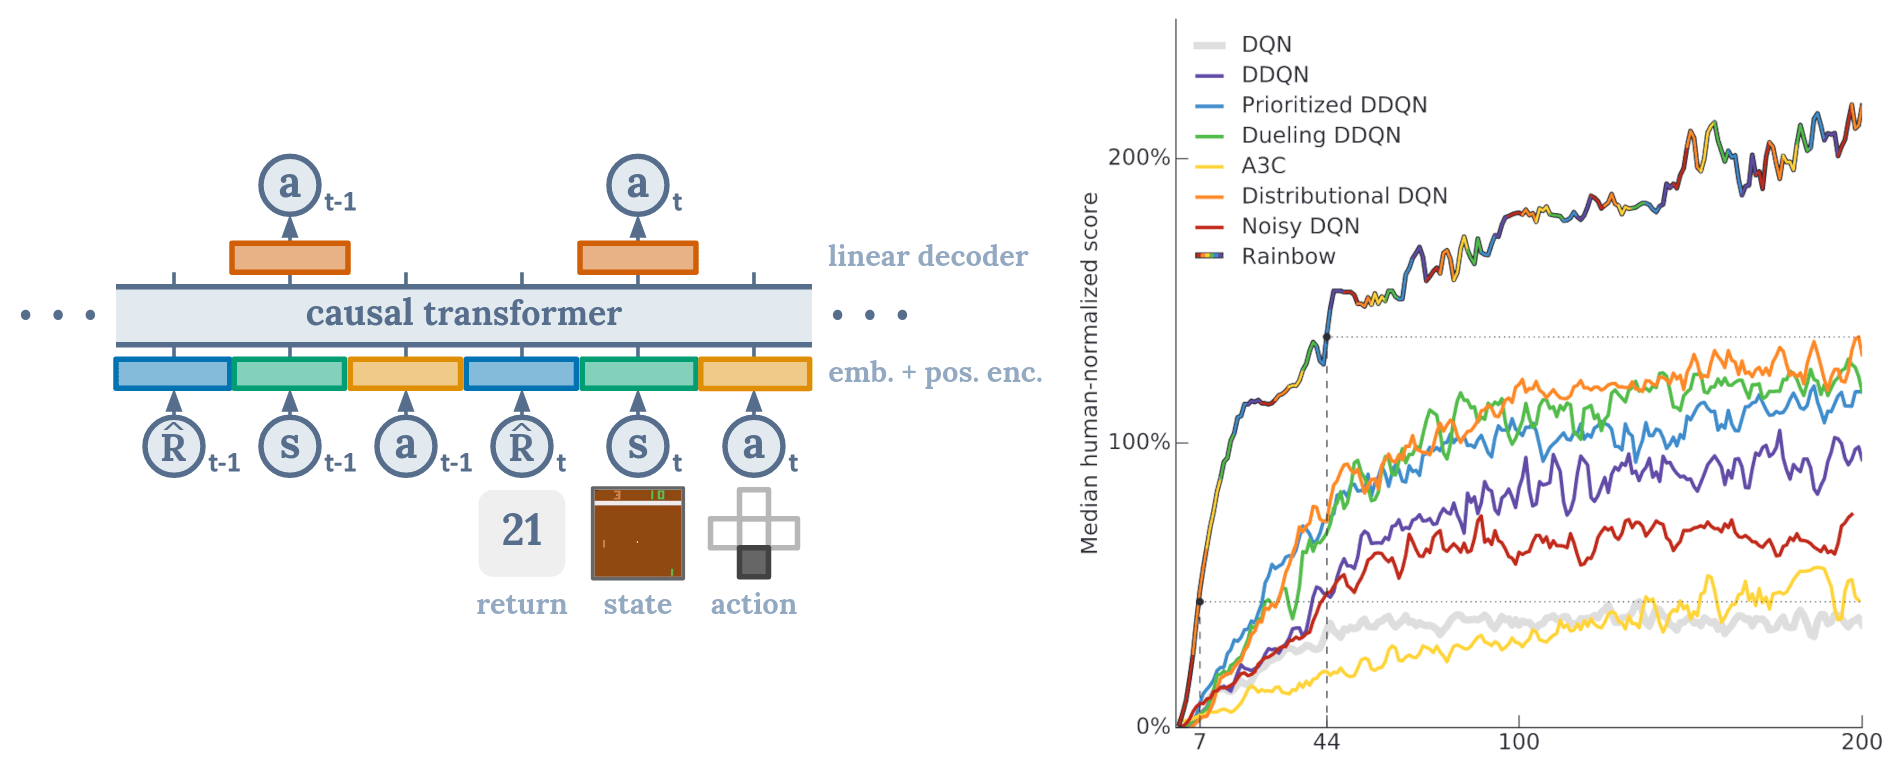
\includegraphics[width=\textwidth]{images/decision-transformer-rainbow.png}
\caption{On the left, the Decision Transformer architecture \cite{decision_transformer}. On the right, Rainbow (discussed later, see \nameref{subsec:rainbow}) performance on the Atari benchmark compared to its single components \cite{rainbow}.}
\label{fig:rainbow}
\end{figure}
